\subsection{Web client}

The web client requires a persistent internet connection and is making all changes in real-time. You are required to log in before using the web client. You will however create a new user, if you enter an email address not already known.

\begin{figure}[htb]
	\centering
	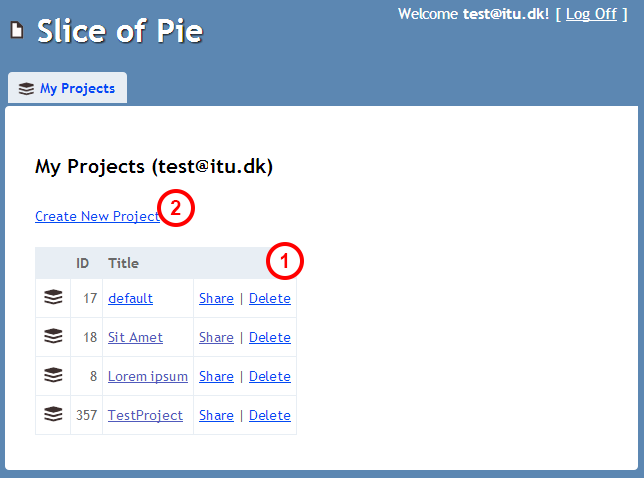
\includegraphics[width=1\textwidth]{User_manual/graphics/web.png}
	\caption{Screenshot of the web client}
	\label{fig:manual-web}
\end{figure}

\subsubsection{Projects}

	\paragraph{Create project}
	To create a new project, click the Create New Project button (2 in figure~\ref{fig:manual-web}) and enter the desired name on the new page. Your new project is now open and you can access an overview of folders and documents (like seen at 1 in figure~\ref{fig:manual-web}).

	\paragraph{Share project}
	To share a project, click the Share button in the overview (1 in figure~\ref{fig:manual-web}). This will lead you to a new page with a text area, which can handle both single email addresses or comma-separated email addresses.
	
	\paragraph{Remove project}
	To remove a project, click the Delete button in the overview (1 in figure~\ref{fig:manual-web}) and confirm. Be aware that all folders, sub folders and documents will also be removed.

\subsubsection{Folders}

	\paragraph{Create folder}
	In order to create a new folder, you have to be inside a project or another folder, from where you can click the Create New Folder button (like seen at 2 in figure~\ref{fig:manual-web}). Then enter the desired name on the new page. Your new folder is now open and you can access a list of folders and documents (like seen at 1 in figure~\ref{fig:manual-web}).

	\paragraph{Remove folder}
	To remove a folder, click the Delete button in the overview (1 in figure~\ref{fig:manual-web}) and confirm. Be aware that all sub folders and documents will also be removed.

\subsubsection{Documents}
	
	\begin{figure}[htb]
		\centering
		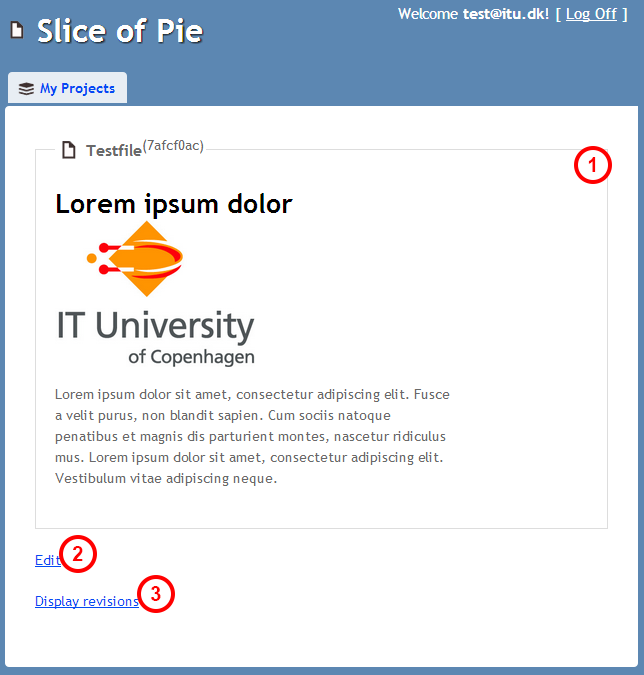
\includegraphics[width=1\textwidth]{User_manual/graphics/web-document.png}
		\caption{Screenshot of the document view in the web client}
		\label{fig:manual-web-document}
	\end{figure}

	\paragraph{View document}
	To view a document, click the Show button in the overview (same location as the Share button in 1 in figure~\ref{fig:manual-web}). This will open a new page with the contents of the document formatted as HTML (1 in figure~\ref{fig:manual-web-document}).
		
		\subparagraph{Show history}
		To view the revisions of a document, click the Display revisions button (3 in figure~\ref{fig:manual-web-document}) in the view of the document. This will show the revisions below the view of the document in a list with latest revision at the top.

	\paragraph{Create document}
	In order to create a new document, you have to be inside a project or another folder, from where you can click the Create New Document button (like seen at 2 in figure~\ref{fig:manual-web}). Then enter the desired name on the new page. Your new document is now open in editing mode.
	
	\paragraph{Edit document}
	To edit a document, either click on the document name in the overview (1 in figure~\ref{fig:manual-web}) or click the Edit button (2 in figure~\ref{fig:manual-web-document}) in the view of the document. When editing the document, you can use the \emph{HyperText markup language}\cite{w3cHTML} (HTML) to format your content. To save the document, click the Edit button below the text box.
	
	\paragraph{Remove document}
	To remove a document, click the Delete button in the overview (1 in figure ~\ref{fig:manual-web}) and confirm. Be aware that all revisions will also be removed.
